\documentclass[]{article}
\usepackage[margin=2cm]{geometry}

%opening
\title{Exercises Set: Linear Algebra\\ \large Solutions}
\author{DSBA Mathematics Refresher 2026}
\date{}

\usepackage{amsmath}
\usepackage{amsfonts}
\usepackage{amsthm}
\usepackage{amssymb}
\usepackage{mathrsfs}
\usepackage{stmaryrd}
\usepackage{tikz}

\newcommand{\Q}{\mathbb{Q}}
\newcommand{\N}{\mathbb{N}}
\newcommand{\Z}{\mathbb{Z}}
\newcommand{\R}{\mathbb{R}}
\newcommand{\Primes}{\mathbb{P}}
\newcommand{\st}{\text{ s.t. }}
\newcommand{\txtand}{\text{ and }}
\newcommand{\txtor}{\text{ or }}
\newcommand{\lxor}{\veebar}


\begin{document}

	\maketitle

	\section{Systems of Linear Equations}
	\paragraph{Reduced Row Echelon Form}\mbox{}

	We row-reduce
	$$\begin{pmatrix}
		1 & 2 & 3 & 4\\
		0 & 6 & 2 & 3\\
		0 & 0 & 0 & 10
	\end{pmatrix}$$

	First, normalize the pivots, with $L_2 \leftarrow \frac{1}{6} L_2$ and $L_3 \leftarrow \frac{1}{10} L_3$:
	$$\begin{pmatrix}
		1 & 2 & 3 & 4\\
		0 & 1 & \frac{1}{3} & \frac{1}{2}\\
		0 & 0 & 0 & 1
	\end{pmatrix}$$

	Then clear the entries above the pivot of $L_2$, with $L_1 \leftarrow L_1 - 2 L_2$:
	$$\begin{pmatrix}
		1 & 0 & \frac{7}{3} & 3\\
		0 & 1 & \frac{1}{3} & \frac{1}{2}\\
		0 & 0 & 0 & 1
	\end{pmatrix}$$

	Finally, clear the entries above the pivot of $L_3$, with $L_1 \leftarrow L_1 - 3 L_3$ and $L_2 \leftarrow L_2 - \frac{1}{2} L_3$:
	$$\begin{pmatrix}
		1 & 0 & \frac{7}{3} & 0\\
		0 & 1 & \frac{1}{3} & 0\\
		0 & 0 & 0 & 1
	\end{pmatrix}$$
	which is the Reduced Row Echelon Form (pivots in columns 1, 2 and 4; column 3 is free).

	\paragraph{Gaussian Elimination (*)}\mbox{}

	The system
	$$\begin{cases}
		2x + y &= 4 \\
		3x + 2y + z &= 5 \\
		y + 3z &= 7
	\end{cases}$$
	has augmented matrix
	$$\left(\begin{array}{ccc|c}
		2 & 1 & 0 & 4\\
		3 & 2 & 1 & 5\\
		0 & 1 & 3 & 7
	\end{array}\right)$$

	With $L_1 \leftarrow \frac{1}{2} L_1$:
	$$\left(\begin{array}{ccc|c}
		1 & \frac{1}{2} & 0 & 2\\
		3 & 2 & 1 & 5\\
		0 & 1 & 3 & 7
	\end{array}\right)$$

	With $L_2 \leftarrow L_2 - 3 L_1$:
	$$\left(\begin{array}{ccc|c}
		1 & \frac{1}{2} & 0 & 2\\
		0 & \frac{1}{2} & 1 & -1\\
		0 & 1 & 3 & 7
	\end{array}\right)$$

	With $L_2 \leftarrow 2 L_2$, then $L_3 \leftarrow L_3 - L_2$:
	$$\left(\begin{array}{ccc|c}
		1 & \frac{1}{2} & 0 & 2\\
		0 & 1 & 2 & -2\\
		0 & 1 & 3 & 7
	\end{array}\right)
	\qquad \longrightarrow \qquad
	\left(\begin{array}{ccc|c}
		1 & \frac{1}{2} & 0 & 2\\
		0 & 1 & 2 & -2\\
		0 & 0 & 1 & 9
	\end{array}\right)$$

	The matrix is now in row echelon form, and we can back-substitute:
	$$z = 9, \qquad y = -2 - 2z = -20, \qquad x = 2 - \tfrac{1}{2} y = 2 + 10 = 12$$

	$$\boxed{x = 12, \quad y = -20, \quad z = 9}$$

	\textit{Check:} $2(12) + (-20) = 4$ \checkmark, \ $3(12) + 2(-20) + 9 = 36 - 40 + 9 = 5$ \checkmark, \ $-20 + 3(9) = 7$. \checkmark


	\section{Vector Spaces}
	\paragraph{Linear Independence}\mbox{}

	Suppose $\lambda_1 \mathbf{v_1} + \lambda_2 \mathbf{v_2} + \lambda_3 \mathbf{v_3} = \mathbf{0}$, with $\lambda_1, \lambda_2, \lambda_3 \in \R$. Component by component:
	$$\begin{cases}
		\lambda_1 + 3\lambda_3 &= 0 \\
		2\lambda_1 + \lambda_2 + 5\lambda_3 &= 0 \\
		2\lambda_3 &= 0
	\end{cases}$$
	The third equation gives $\lambda_3 = 0$; the first then gives $\lambda_1 = 0$; and the second finally gives $\lambda_2 = 0$.

	The only linear combination of $\mathbf{v_1}, \mathbf{v_2}, \mathbf{v_3}$ equal to $\mathbf{0}$ is the trivial one, so they are linearly independent.

	Since they are $3$ linearly independent vectors in $\R^3$, they also span $\R^3$: they form a basis of $\R^3$.

	\paragraph{Space of Polynomials}\mbox{}

	Let $q \in \Primes_2$, say $q(x) = a x^2 + b x + c$ with $a, b, c \in \R$. Since $3x^2 - 1 = p_3(x)$, we have $x^2 = \frac{1}{3}\left(p_3(x) + 1\right)$, and therefore
	\begin{align*}
		q(x) &= a x^2 + b x + c \\
		     &= \frac{a}{3}\left(3x^2 - 1\right) + \frac{a}{3} + \frac{b}{2}\left(2x\right) + c \\
		     &= \frac{a}{3} \, p_3(x) + \frac{b}{2} \, p_2(x) + \left(c + \frac{a}{3}\right) p_1(x)
	\end{align*}

	Any $q \in \Primes_2$ is thus a linear combination of $p_1, p_2, p_3$, so $\{p_1, p_2, p_3\}$ spans $\Primes_2$.

	(They are moreover $3$ vectors spanning the $3$-dimensional space $\Primes_2$, so they form a basis of $\Primes_2$.)


	\section{Matrix Inverses}
	\paragraph{2x2 Matrices}\mbox{}

	For $A = \begin{bmatrix} 2 & 1 \\ 0 & 2 \end{bmatrix}$, we have $\det(A) = 2 \cdot 2 - 1 \cdot 0 = 4 \neq 0$, so $A$ is invertible, and using the formula for $2 \times 2$ matrices:
	$$A^{-1} = \frac{1}{\det(A)} \begin{bmatrix} 2 & -1 \\ 0 & 2 \end{bmatrix} = \frac{1}{4} \begin{bmatrix} 2 & -1 \\ 0 & 2 \end{bmatrix} = \begin{bmatrix} \frac{1}{2} & -\frac{1}{4} \\ 0 & \frac{1}{2} \end{bmatrix}$$

	\textit{Check:}
	$$A A^{-1} = \begin{bmatrix} 2 & 1 \\ 0 & 2 \end{bmatrix} \begin{bmatrix} \frac{1}{2} & -\frac{1}{4} \\ 0 & \frac{1}{2} \end{bmatrix} = \begin{bmatrix} 1 & -\frac{1}{2} + \frac{1}{2} \\ 0 & 1 \end{bmatrix} = I_2
	\qquad \text{and likewise} \qquad A^{-1} A = I_2 \ \checkmark$$

	\paragraph{3x3 Matrices (*)}\mbox{}

	For $B = \begin{bmatrix} 0 & 1 & 3 \\ 1 & 2 & 0 \\ -1 & 0 & 1 \end{bmatrix}$, expanding the determinant along the first row:
	$$\det(B) = 0 \cdot (2 \cdot 1 - 0 \cdot 0) - 1 \cdot (1 \cdot 1 - 0 \cdot (-1)) + 3 \cdot (1 \cdot 0 - 2 \cdot (-1)) = 0 - 1 + 6 = 5 \neq 0$$
	so $B$ is invertible. We find $B^{-1}$ by Gauss-Jordan elimination on $\left(B \mid I_3\right)$:
	$$\left(\begin{array}{ccc|ccc}
		0 & 1 & 3 & 1 & 0 & 0\\
		1 & 2 & 0 & 0 & 1 & 0\\
		-1 & 0 & 1 & 0 & 0 & 1
	\end{array}\right)
	\quad \xrightarrow{\ L_1 \leftrightarrow L_2 \ }\quad
	\left(\begin{array}{ccc|ccc}
		1 & 2 & 0 & 0 & 1 & 0\\
		0 & 1 & 3 & 1 & 0 & 0\\
		-1 & 0 & 1 & 0 & 0 & 1
	\end{array}\right)$$

	$$\xrightarrow{\ L_1 \leftarrow L_1 - 2L_2 \ }\quad
	\left(\begin{array}{ccc|ccc}
		1 & 0 & -6 & -2 & 1 & 0\\
		0 & 1 & 3 & 1 & 0 & 0\\
		-1 & 0 & 1 & 0 & 0 & 1
	\end{array}\right)
	\quad \xrightarrow{\ L_3 \leftarrow L_3 + L_1 \ }\quad
	\left(\begin{array}{ccc|ccc}
		1 & 0 & -6 & -2 & 1 & 0\\
		0 & 1 & 3 & 1 & 0 & 0\\
		0 & 0 & -5 & -2 & 1 & 1
	\end{array}\right)$$

	$$\xrightarrow{\ L_3 \leftarrow -\frac{1}{5} L_3 \ }\quad
	\left(\begin{array}{ccc|ccc}
		1 & 0 & -6 & -2 & 1 & 0\\
		0 & 1 & 3 & 1 & 0 & 0\\
		0 & 0 & 1 & \frac{2}{5} & -\frac{1}{5} & -\frac{1}{5}
	\end{array}\right)
	\quad \xrightarrow[\ L_2 \leftarrow L_2 - 3L_3 \ ]{\ L_1 \leftarrow L_1 + 6L_3 \ }\quad
	\left(\begin{array}{ccc|ccc}
		1 & 0 & 0 & \frac{2}{5} & -\frac{1}{5} & -\frac{6}{5}\\
		0 & 1 & 0 & -\frac{1}{5} & \frac{3}{5} & \frac{3}{5}\\
		0 & 0 & 1 & \frac{2}{5} & -\frac{1}{5} & -\frac{1}{5}
	\end{array}\right)$$

	The left block is $I_3$, and therefore
	$$B^{-1} = \frac{1}{5} \begin{bmatrix} 2 & -1 & -6 \\ -1 & 3 & 3 \\ 2 & -1 & -1 \end{bmatrix}$$
	(it is common to factor $\frac{1}{\det(B)}$ out in front of $B^{-1}$).

	\textit{Check:}
	$$B B^{-1} = \frac{1}{5} \begin{bmatrix} 0 & 1 & 3 \\ 1 & 2 & 0 \\ -1 & 0 & 1 \end{bmatrix} \begin{bmatrix} 2 & -1 & -6 \\ -1 & 3 & 3 \\ 2 & -1 & -1 \end{bmatrix}
	= \frac{1}{5} \begin{bmatrix} 5 & 0 & 0 \\ 0 & 5 & 0 \\ 0 & 0 & 5 \end{bmatrix} = I_3
	\qquad \text{and likewise} \qquad B^{-1} B = I_3 \ \checkmark$$


	\section{Eigenvalues and Eigenvectors}
	\paragraph{Basic 2x2 Case (*)}\mbox{}

	For $A = \begin{bmatrix} 3 & 1 \\ 1 & 3 \end{bmatrix}$, the characteristic polynomial is
	\begin{align*}
		\mathrm{ch}_A(\lambda) = \det\left(A - \lambda I_2\right) = (3 - \lambda)^2 - 1 = \lambda^2 - 6\lambda + 8
	\end{align*}
	With $\Delta = 36 - 32 = 4$, the roots are $\lambda = \dfrac{6 \pm 2}{2}$, so the eigenvalues are $\lambda_1 = 2$ and $\lambda_2 = 4$.

	\textit{For $\lambda_1 = 2$:} $A \mathbf{x} = 2 \mathbf{x}$ reads
	$$\begin{cases} 3x + y = 2x \\ x + 3y = 2y \end{cases} \quad \Longleftrightarrow \quad x + y = 0$$
	Setting $x = 1$ gives $y = -1$, so an eigenvector is $\mathbf{x_1} = \begin{bmatrix} 1 \\ -1 \end{bmatrix}$.

	\textit{For $\lambda_2 = 4$:} $A \mathbf{x} = 4 \mathbf{x}$ reads
	$$\begin{cases} 3x + y = 4x \\ x + 3y = 4y \end{cases} \quad \Longleftrightarrow \quad x = y$$
	Setting $x = 1$ gives $y = 1$, so an eigenvector is $\mathbf{x_2} = \begin{bmatrix} 1 \\ 1 \end{bmatrix}$.

	\begin{center}
		\begin{tikzpicture}[scale=0.72]
			\draw[->] (-4.4,0) -- (4.4,0) node[right] {\scriptsize $x$};
			\draw[->] (0,-4.4) -- (0,4.4) node[above] {\scriptsize $y$};
			\draw[dashed,gray] (0,0) circle (1);
			\draw[rotate=45] (0,0) ellipse (4 and 2);
			% a generic vector and its image: direction changes
			\draw[->,gray!80] (0,0) -- (1,0);
			\draw[->,gray!80,dashed] (0,0) -- (3,1);
			\node[gray!80,below right] at (3.05,0.92) {\scriptsize $A\mathbf{v}$};
			\node[gray!80,below] at (1.02,-0.04) {\scriptsize $\mathbf{v}$};
			% eigenvectors: direction preserved
			\draw[->,very thick] (0,0) -- (0.7071,0.7071);
			\draw[->,thick] (0.7071,0.7071) -- (2.828,2.828);
			\node[above right] at (2.85,2.86) {\scriptsize $\times 4$};
			\node[left] at (0.60,0.86) {\scriptsize $\mathbf{x_2}$};
			\draw[->,very thick] (0,0) -- (0.7071,-0.7071);
			\draw[->,thick] (0.7071,-0.7071) -- (1.414,-1.414);
			\node[below right] at (1.44,-1.44) {\scriptsize $\times 2$};
			\node[right] at (0.80,-0.60) {\scriptsize $\mathbf{x_1}$};
		\end{tikzpicture}
	\end{center}
	Multiplying by $A$ turns the dashed unit circle into the ellipse.
	A generic vector such as $\mathbf{v} = \binom{1}{0}$ changes \textit{direction} (grey), but the two eigenvectors do not: they are only stretched, by $4$ and by $2$ --- and those factors are precisely the eigenvalues.
	The ellipse's axes lie along them.

	\paragraph{Repeated Eigenvalues}\mbox{}

	For $B = \begin{bmatrix} 1 & -1 \\ 0 & 1 \end{bmatrix}$:
	$$\mathrm{ch}_B(\lambda) = \det\begin{pmatrix} 1 - \lambda & -1 \\ 0 & 1 - \lambda \end{pmatrix} = (1-\lambda)^2 - 0 \cdot (-1) = (1 - \lambda)^2$$
	so $\lambda = 1$ is the only eigenvalue, with multiplicity $2$.

	$B \mathbf{x} = 1 \cdot \mathbf{x}$ reads
	$$\begin{cases} x - y = x \\ y = y \end{cases} \quad \Longleftrightarrow \quad y = 0$$
	Setting $x = 1$, the only eigenvectors are the multiples of $\mathbf{x_1} = \begin{bmatrix} 1 \\ 0 \end{bmatrix}$: the eigenvalue has algebraic multiplicity $2$ but geometric multiplicity $1$.

	(For a \textit{generalized} eigenvector, one solves $(B - \lambda I)\mathbf{x} = \mathbf{x_1}$ instead of $(B - \lambda I)\mathbf{x} = \mathbf{0}$:
	$$\begin{cases} 0 \cdot x - y = 1 \\ 0 \cdot x + 0 \cdot y = 0 \end{cases} \quad \Longrightarrow \quad y = -1$$
	and setting $x = 0$ gives $\mathbf{x_2} = \begin{bmatrix} 0 \\ -1 \end{bmatrix}$.)

	\paragraph{Basic 3x3 Case}\mbox{}

	For $C = \begin{bmatrix} 1 & 2 & 0 \\ 0 & 2 & 0 \\ 0 & 1 & 3 \end{bmatrix}$, the matrix $C - \lambda I_3$ is lower-triangular up to the zeros in the last column, and expanding the determinant gives
	$$\mathrm{ch}_C(\lambda) = (1 - \lambda)(2 - \lambda)(3 - \lambda)$$
	so the eigenvalues are $\lambda = 1$, $\lambda = 2$ and $\lambda = 3$.

	\textit{For $\lambda = 1$:} $C\mathbf{x} = \mathbf{x}$ reads
	$$\begin{cases} x + 2y = x \\ 2y = y \\ y + 3z = z \end{cases} \quad \Longrightarrow \quad y = 0 \ \text{ and } \ z = 0$$
	Setting $x = 1$: $\mathbf{x} = \begin{bmatrix} 1 \\ 0 \\ 0 \end{bmatrix}$.

	\textit{For $\lambda = 2$:} $C\mathbf{x} = 2\mathbf{x}$ reads
	$$\begin{cases} x + 2y = 2x \\ 2y = 2y \\ y + 3z = 2z \end{cases} \quad \Longrightarrow \quad x = 2y \ \text{ and } \ z = -y$$
	Setting $y = 1$: $\mathbf{x} = \begin{bmatrix} 2 \\ 1 \\ -1 \end{bmatrix}$.

	\textit{For $\lambda = 3$:} $C\mathbf{x} = 3\mathbf{x}$ reads
	$$\begin{cases} x + 2y = 3x \\ 2y = 3y \\ y + 3z = 3z \end{cases} \quad \Longrightarrow \quad y = 0 \ \text{ and } \ x = 0$$
	Setting $z = 1$: $\mathbf{x} = \begin{bmatrix} 0 \\ 0 \\ 1 \end{bmatrix}$.


	\section{Diagonalization}

	\paragraph{Matrix $A$}\mbox{}

	$A$ has $2$ distinct eigenvalues, hence $2$ linearly independent eigenvectors: it is diagonalizable, with $A = P D P^{-1}$ where
	$$D = \begin{bmatrix} 2 & 0 \\ 0 & 4 \end{bmatrix} \quad \text{(the eigenvalues)}, \qquad
	P = \begin{bmatrix} 1 & 1 \\ -1 & 1 \end{bmatrix} \quad \text{(the corresponding eigenvectors, as columns)}$$
	Using the formula for the inverse of a $2 \times 2$ matrix, $\det(P) = 2$ and
	$$P^{-1} = \frac{1}{2} \begin{bmatrix} 1 & -1 \\ 1 & 1 \end{bmatrix}$$
	One may check that $P D P^{-1}$ is indeed $A$:
	$$P D P^{-1} = \frac{1}{2}\begin{bmatrix} 1 & 1 \\ -1 & 1 \end{bmatrix} \begin{bmatrix} 2 & 0 \\ 0 & 4 \end{bmatrix} \begin{bmatrix} 1 & -1 \\ 1 & 1 \end{bmatrix}
	= \frac{1}{2}\begin{bmatrix} 2 & 4 \\ -2 & 4 \end{bmatrix} \begin{bmatrix} 1 & -1 \\ 1 & 1 \end{bmatrix}
	= \frac{1}{2}\begin{bmatrix} 6 & 2 \\ 2 & 6 \end{bmatrix} = A \ \checkmark$$

	\paragraph{Matrix $B$}\mbox{}

	$B$ is \textbf{not} diagonalizable: all its eigenvectors are multiples of $\begin{bmatrix} 1 \\ 0 \end{bmatrix}$, so it does not have $2$ linearly independent eigenvectors.

	\paragraph{Matrix $C$}\mbox{}

	$C$ has $3$ distinct eigenvalues, hence $3$ linearly independent eigenvectors: it is diagonalizable, with $C = P D P^{-1}$ where
	$$P = \begin{bmatrix} 1 & 2 & 0 \\ 0 & 1 & 0 \\ 0 & -1 & 1 \end{bmatrix}, \qquad
	D = \begin{bmatrix} 1 & 0 & 0 \\ 0 & 2 & 0 \\ 0 & 0 & 3 \end{bmatrix}$$
	and one may find (by Gauss-Jordan elimination on $\left(P \mid I_3\right)$)
	$$P^{-1} = \begin{bmatrix} 1 & -2 & 0 \\ 0 & 1 & 0 \\ 0 & 1 & 1 \end{bmatrix}$$


	\section{Orthogonal Vectors}
	\paragraph{Orthogonality}\mbox{}

	\begin{align*}
		\mathbf{u} \cdot \mathbf{v} &= 2 \cdot 1 + (-1) \cdot 2 + 0 \cdot 1 = 0 &&\Longrightarrow \quad \mathbf{u} \perp \mathbf{v} \\
		\mathbf{u} \cdot \mathbf{w} &= 2 \cdot 0 + (-1) \cdot 1 + 0 \cdot (-2) = -1 &&\Longrightarrow \quad \mathbf{u} \not\perp \mathbf{w} \\
		\mathbf{v} \cdot \mathbf{w} &= 1 \cdot 0 + 2 \cdot 1 + 1 \cdot (-2) = 0 &&\Longrightarrow \quad \mathbf{v} \perp \mathbf{w}
	\end{align*}

	So $\mathbf{u} \perp \mathbf{v}$ and $\mathbf{v} \perp \mathbf{w}$, but $\mathbf{u}$ and $\mathbf{w}$ are not orthogonal.

	\paragraph{Gram-Schmidt Orthogonalization (*)}\mbox{}

	Write $\mathbf{v}_1 = \begin{bmatrix} 1 \\ 2 \end{bmatrix}$ and $\mathbf{v}_2 = \begin{bmatrix} 0 \\ 1 \end{bmatrix}$.

	\textit{First vector:} $\|\mathbf{v}_1\| = \sqrt{1^2 + 2^2} = \sqrt{5}$, so
	$$\mathbf{u}_1 = \frac{\mathbf{v}_1}{\|\mathbf{v}_1\|} = \frac{1}{\sqrt{5}} \begin{bmatrix} 1 \\ 2 \end{bmatrix} = \begin{bmatrix} \frac{\sqrt{5}}{5} \\ \frac{2\sqrt{5}}{5} \end{bmatrix}$$

	\textit{Second vector:} we remove from $\mathbf{v}_2$ its component along $\mathbf{u}_1$. Since $\mathbf{v}_2 \cdot \mathbf{u}_1 = \dfrac{2}{\sqrt{5}}$,
	$$\tilde{\mathbf{u}}_2 = \mathbf{v}_2 - \left(\mathbf{v}_2 \cdot \mathbf{u}_1\right) \mathbf{u}_1
	= \begin{bmatrix} 0 \\ 1 \end{bmatrix} - \frac{2}{\sqrt{5}} \cdot \frac{1}{\sqrt{5}} \begin{bmatrix} 1 \\ 2 \end{bmatrix}
	= \begin{bmatrix} 0 \\ 1 \end{bmatrix} - \frac{2}{5} \begin{bmatrix} 1 \\ 2 \end{bmatrix}
	= \begin{bmatrix} -\frac{2}{5} \\ \frac{1}{5} \end{bmatrix}$$
	and $\|\tilde{\mathbf{u}}_2\| = \sqrt{\dfrac{4}{25} + \dfrac{1}{25}} = \dfrac{1}{\sqrt{5}}$, so
	$$\mathbf{u}_2 = \frac{\tilde{\mathbf{u}}_2}{\|\tilde{\mathbf{u}}_2\|} = \sqrt{5} \begin{bmatrix} -\frac{2}{5} \\ \frac{1}{5} \end{bmatrix} = \begin{bmatrix} -\frac{2\sqrt{5}}{5} \\ \frac{\sqrt{5}}{5} \end{bmatrix}$$

	\begin{center}
		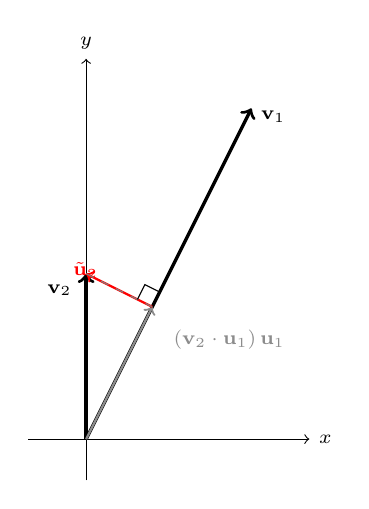
\begin{tikzpicture}[scale=2.1]
			\draw[->] (-0.35,0) -- (1.35,0) node[right] {\scriptsize $x$};
			\draw[->] (0,-0.25) -- (0,2.3) node[above] {\scriptsize $y$};
			\draw[->,very thick] (0,0) -- (1,2);
			\node[right] at (1.0,1.95) {\scriptsize $\mathbf{v}_1$};
			\draw[->,very thick] (0,0) -- (0,1);
			\node[left] at (-0.03,0.9) {\scriptsize $\mathbf{v}_2$};
			\draw[->,thick,gray!90] (0,0) -- (0.4,0.8);
			\node[gray!90,right] at (0.47,0.60) {\scriptsize $\left(\mathbf{v}_2\cdot\mathbf{u}_1\right)\mathbf{u}_1$};
			\draw[->,thick,red] (0.4,0.8) -- (0,1);
			\node[red,left] at (0.13,1.02) {\scriptsize $\tilde{\mathbf{u}}_2$};
			\draw[dashed,gray] (0,1) -- (0.4,0.8);
			% right angle marker at the foot of the projection
			\draw (0.4,0.8) ++(-0.0894,0.0447) -- ++(0.0447,0.0894) -- ++(0.0894,-0.0447);
		\end{tikzpicture}
	\end{center}
	The construction in one picture: we slide down the component of $\mathbf{v}_2$ that lies \textit{along} $\mathbf{v}_1$ (grey), and what is left over (red) is perpendicular to it by construction.
	Normalizing the two thick directions gives $\mathbf{u}_1$ and $\mathbf{u}_2$.

	$\{\mathbf{u}_1, \mathbf{u}_2\}$ is an orthonormal basis of the span of $\{\mathbf{v}_1, \mathbf{v}_2\}$, which here is all of $\R^2$.

	\textit{Verification:}
	$$\|\mathbf{u}_1\| = \sqrt{\frac{5}{25} + \frac{20}{25}} = \sqrt{\frac{25}{25}} = 1, \qquad
	\|\mathbf{u}_2\| = \sqrt{\frac{20}{25} + \frac{5}{25}} = 1$$
	$$\mathbf{u}_1 \cdot \mathbf{u}_2 = \frac{\sqrt{5}}{5} \cdot \left(-\frac{2\sqrt{5}}{5}\right) + \frac{2\sqrt{5}}{5} \cdot \frac{\sqrt{5}}{5} = -\frac{10}{25} + \frac{10}{25} = 0 \ \checkmark$$


	\section{Norms}

	With $\mathbf{v} = \begin{pmatrix} 1 \\ -2 \\ 3 \end{pmatrix}$ and $\mathbf{w} = \begin{pmatrix} -1 \\ 4 \\ -2 \end{pmatrix}$, we have $\mathbf{v} + \mathbf{w} = \begin{pmatrix} 0 \\ 2 \\ 1 \end{pmatrix}$, and
	$$\|\mathbf{v} + \mathbf{w}\|_1 = 0 + 2 + 1 = 3, \qquad \|\mathbf{v}\|_1 = 1 + 2 + 3 = 6, \qquad \|\mathbf{w}\|_1 = 1 + 4 + 2 = 7$$
	so
	$$\|\mathbf{v} + \mathbf{w}\|_1 = 3 \ \leq \ 13 = 6 + 7 = \|\mathbf{v}\|_1 + \|\mathbf{w}\|_1 \ \checkmark$$

	Now with the error vector $\mathbf{v} = \begin{pmatrix} -0.1 \\ 0.05 \\ 0.2 \end{pmatrix}$:
	\begin{enumerate}
		\item $\|\mathbf{v}\|_1 = 0.1 + 0.05 + 0.2 = 0.35$
		\item $\|\mathbf{v}\|_2 = \sqrt{0.01 + 0.0025 + 0.04} = \sqrt{0.0525} \approx 0.229$
		\item[] \mbox{}\\
		\begin{center}
			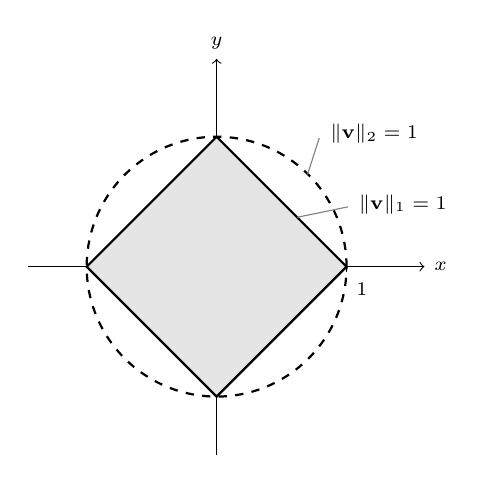
\begin{tikzpicture}[scale=1.65]
				\draw[->] (-1.45,0) -- (1.6,0) node[right] {\scriptsize $x$};
				\draw[->] (0,-1.45) -- (0,1.6) node[above] {\scriptsize $y$};
				\fill[gray!20] (1,0) -- (0,1) -- (-1,0) -- (0,-1) -- cycle;
				\draw[thick] (1,0) -- (0,1) -- (-1,0) -- (0,-1) -- cycle;
				\draw[thick,dashed] (0,0) circle (1);
				\node[right] at (0.80,1.02) {\scriptsize $\|\mathbf{v}\|_2 = 1$};
				\draw[gray] (0.79,0.99) -- (0.70,0.71);
				\node[right] at (1.02,0.48) {\scriptsize $\|\mathbf{v}\|_1 = 1$};
				\draw[gray] (1.01,0.46) -- (0.62,0.38);
				\draw (1,0.04) -- (1,-0.04); \node[below right] at (1.0,-0.05) {\scriptsize $1$};
			\end{tikzpicture}
		\end{center}
		The two "unit balls": the set of vectors of $L_1$ norm $1$ (the diamond) sits \textit{inside} the set of vectors of $L_2$ norm $1$ (the circle).
		Along the axes the two norms agree; away from them the $L_1$ norm is the larger of the two, which is why $\|\mathbf{v}\|_2 \leq \|\mathbf{v}\|_1$ always.

		\item The $L_1$ norm is the Manhattan distance: it simply adds up the individual errors, so every component contributes proportionally to its size. The $L_2$ norm is the Euclidean distance: because the errors are squared, large errors weigh much more than small ones.

		In practice, an $L_1$ loss is more robust to outliers and easier to interpret (it is the total absolute error), while an $L_2$ loss penalizes large errors much more heavily, and so pushes the model to avoid big mistakes even at the cost of many small ones. Depending on the context, one may be more appropriate than the other.
	\end{enumerate}

\end{document}
